\documentclass[crop=false]{standalone}
%\documentclass{standalone}
\usepackage{tikz} % To generate the plot from csv
\usepackage{pgfplots}
\usepackage{graphicx}
\usepackage{booktabs}
\usepackage{subfig}
\usepackage{float}
\usepackage[section]{placeins} % getting figures below sections
\usepackage{blindtext}
\usepackage{siunitx}
\usepgfplotslibrary{units} % Allows to enter the units nicely
\usetikzlibrary{external} %https://tex.stackexchange.com/questions/1460/script-to-automate-externalizing-tikz-graphics
\tikzexternalize[prefix=savedfigures/]

\pgfplotsset{compat=newest} % Allows to place the legend below plot
\usepackage{pgfplotstable}
\usepgfplotslibrary{statistics}

% #################### Function definition for box plots read table ##################\
\makeatletter
\pgfplotsset{
	boxplot prepared from table/.code={
		\def\tikz@plot@handler{\pgfplotsplothandlerboxplotprepared}%
		\pgfplotsset{
			/pgfplots/boxplot prepared from table/.cd,
			#1,
		}
	},
	/pgfplots/boxplot prepared from table/.cd,
	table/.code={\pgfplotstablecopy{#1}\to\boxplot@datatable},
	row/.initial=0,
	make style readable from table/.style={
		#1/.code={
			\pgfplotstablegetelem{\pgfkeysvalueof{/pgfplots/boxplot prepared from table/row}}{##1}\of\boxplot@datatable
			\pgfplotsset{boxplot/#1/.expand once={\pgfplotsretval}}
		}
	},
	make style readable from table=lower whisker,
	make style readable from table=upper whisker,
	make style readable from table=lower quartile,
	make style readable from table=upper quartile,
	make style readable from table=median,
	make style readable from table=average,
	make style readable from table=lower notch,
	make style readable from table=upper notch
}
\makeatother
\begin{document}

\section{23 2 Mumford0 SA Mutations AMALGAM 20210815 221256}

% ######################## UTRP SA Mutation operators applied ######################## 
\begin{figure} 
\centering 
\tikzsetnextfilename{UTRP_DBMOSA_BP_mutation_funcs_Best_comp} 
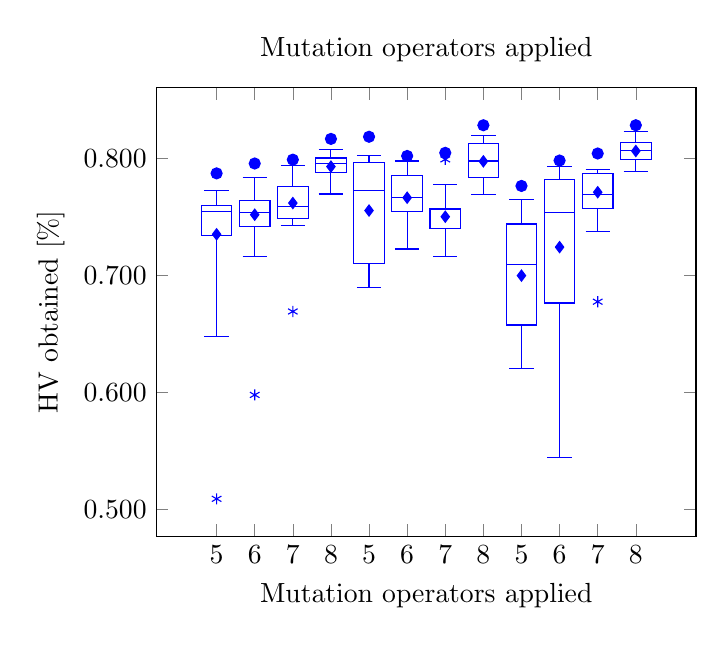
\begin{tikzpicture} 
\begin{axis}[ 
title={Mutation operators applied}, 
boxplot/draw direction=y, 
xtick={1,2,3,4,5,6,7,8,9,10,11,12}, 
xticklabels={5,6,7,8,5,6,7,8,5,6,7,8}, 
x tick label style={rotate=0, align=center}, 
xlabel={Mutation operators applied}, 
y tick label style={/pgf/number format/.cd,fixed,precision=3, zerofill}, 
ylabel={HV obtained [\%]}, 
] 

% ############## B_Mutations_AMALGAM=5 ################## 
\addplot[boxplot, mark=asterisk, 
boxplot prepared={ 
lower whisker=0.64789, 
upper whisker=0.77213, 
lower quartile=0.73402, 
upper quartile=0.7597, 
median=0.75434, 
average=0.73501}, 
color = blue, solid, area legend] 
coordinates {
(1,0.50905)}; 
\addplot[only marks,mark=*,color = blue]coordinates{(1,0.78705)}; 

% ############## B_Mutations_AMALGAM=6 ################## 
\addplot[boxplot, mark=asterisk, 
boxplot prepared={ 
lower whisker=0.71569, 
upper whisker=0.78337, 
lower quartile=0.74183, 
upper quartile=0.76359, 
median=0.75391, 
average=0.75176}, 
color = blue, solid, area legend] 
coordinates {
(2,0.59781)}; 
\addplot[only marks,mark=*,color = blue]coordinates{(2,0.79549)}; 

% ############## B_Mutations_AMALGAM=7 ################## 
\addplot[boxplot, mark=asterisk, 
boxplot prepared={ 
lower whisker=0.74215, 
upper whisker=0.79344, 
lower quartile=0.74824, 
upper quartile=0.77589, 
median=0.75864, 
average=0.7617}, 
color = blue, solid, area legend] 
coordinates {
(3,0.66907)}; 
\addplot[only marks,mark=*,color = blue]coordinates{(3,0.79877)}; 

% ############## B_Mutations_AMALGAM=8 ################## 
\addplot[boxplot, mark=asterisk, 
boxplot prepared={ 
lower whisker=0.76943, 
upper whisker=0.80766, 
lower quartile=0.78783, 
upper quartile=0.80015, 
median=0.79526, 
average=0.79282}, 
color = blue, solid, area legend] 
coordinates {}; 
\addplot[only marks,mark=*,color = blue]coordinates{(4,0.8165)}; 

% ############## B_Mutations_AMALGAM=5 ################## 
\addplot[boxplot, mark=asterisk, 
boxplot prepared={ 
lower whisker=0.6893, 
upper whisker=0.80195, 
lower quartile=0.71031, 
upper quartile=0.7966, 
median=0.77244, 
average=0.75532}, 
color = blue, solid, area legend] 
coordinates {}; 
\addplot[only marks,mark=*,color = blue]coordinates{(5,0.81832)}; 

% ############## B_Mutations_AMALGAM=6 ################## 
\addplot[boxplot, mark=asterisk, 
boxplot prepared={ 
lower whisker=0.72242, 
upper whisker=0.79762, 
lower quartile=0.75485, 
upper quartile=0.78549, 
median=0.76658, 
average=0.76628}, 
color = blue, solid, area legend] 
coordinates {}; 
\addplot[only marks,mark=*,color = blue]coordinates{(6,0.80192)}; 

% ############## B_Mutations_AMALGAM=7 ################## 
\addplot[boxplot, mark=asterisk, 
boxplot prepared={ 
lower whisker=0.71571, 
upper whisker=0.77759, 
lower quartile=0.73995, 
upper quartile=0.75698, 
median=0.75626, 
average=0.75004}, 
color = blue, solid, area legend] 
coordinates {
(7,0.799)}; 
\addplot[only marks,mark=*,color = blue]coordinates{(7,0.80459)}; 

% ############## B_Mutations_AMALGAM=8 ################## 
\addplot[boxplot, mark=asterisk, 
boxplot prepared={ 
lower whisker=0.76866, 
upper whisker=0.81934, 
lower quartile=0.78378, 
upper quartile=0.81284, 
median=0.79763, 
average=0.79736}, 
color = blue, solid, area legend] 
coordinates {}; 
\addplot[only marks,mark=*,color = blue]coordinates{(8,0.82816)}; 

% ############## B_Mutations_AMALGAM=5 ################## 
\addplot[boxplot, mark=asterisk, 
boxplot prepared={ 
lower whisker=0.62038, 
upper whisker=0.7645, 
lower quartile=0.65756, 
upper quartile=0.74382, 
median=0.70934, 
average=0.6997}, 
color = blue, solid, area legend] 
coordinates {}; 
\addplot[only marks,mark=*,color = blue]coordinates{(9,0.77631)}; 

% ############## B_Mutations_AMALGAM=6 ################## 
\addplot[boxplot, mark=asterisk, 
boxplot prepared={ 
lower whisker=0.54466, 
upper whisker=0.79277, 
lower quartile=0.67635, 
upper quartile=0.7817, 
median=0.7536, 
average=0.72407}, 
color = blue, solid, area legend] 
coordinates {}; 
\addplot[only marks,mark=*,color = blue]coordinates{(10,0.79802)}; 

% ############## B_Mutations_AMALGAM=7 ################## 
\addplot[boxplot, mark=asterisk, 
boxplot prepared={ 
lower whisker=0.73766, 
upper whisker=0.79054, 
lower quartile=0.75728, 
upper quartile=0.78691, 
median=0.76928, 
average=0.77094}, 
color = blue, solid, area legend] 
coordinates {
(11,0.67742)}; 
\addplot[only marks,mark=*,color = blue]coordinates{(11,0.80403)}; 

% ############## B_Mutations_AMALGAM=8 ################## 
\addplot[boxplot, mark=asterisk, 
boxplot prepared={ 
lower whisker=0.78859, 
upper whisker=0.82303, 
lower quartile=0.79904, 
upper quartile=0.8138, 
median=0.80677, 
average=0.80617}, 
color = blue, solid, area legend] 
coordinates {}; 
\addplot[only marks,mark=*,color = blue]coordinates{(12,0.82817)}; 

\end{axis}
\end{tikzpicture}
\end{figure} 

% ######################## UTRP SA Mutation operators applied ######################## 
\begin{figure} 
\centering 
\tikzsetnextfilename{UTRP_DBMOSA_BP_mutation_funcs_AMAL} 
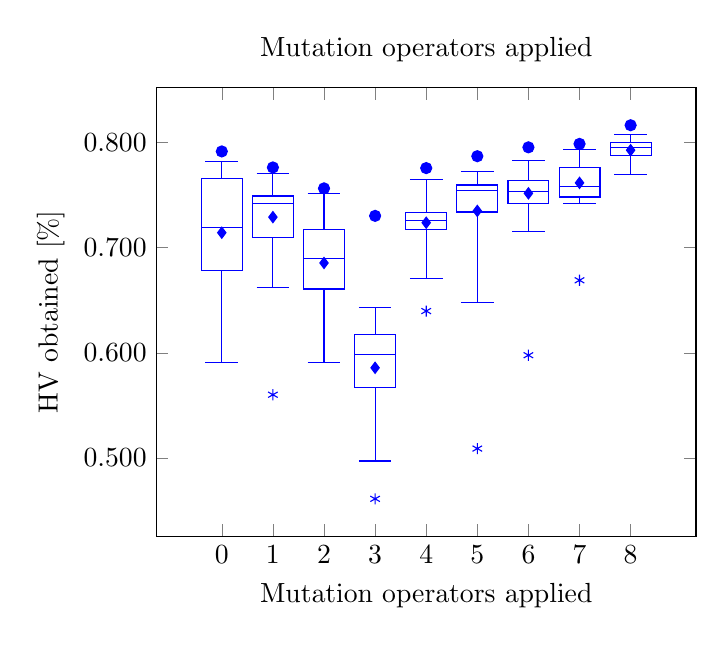
\begin{tikzpicture} 
\begin{axis}[ 
title={Mutation operators applied}, 
boxplot/draw direction=y, 
xtick={1,2,3,4,5,6,7,8,9}, 
xticklabels={0,1,2,3,4,5,6,7,8}, 
x tick label style={rotate=0, align=center}, 
xlabel={Mutation operators applied}, 
y tick label style={/pgf/number format/.cd,fixed,precision=3, zerofill}, 
ylabel={HV obtained [\%]}, 
] 

% ############## Mutations_AMALGAM=0 ################## 
\addplot[boxplot, mark=asterisk, 
boxplot prepared={ 
lower whisker=0.59097, 
upper whisker=0.78204, 
lower quartile=0.67871, 
upper quartile=0.76599, 
median=0.71921, 
average=0.7143}, 
color = blue, solid, area legend] 
coordinates {}; 
\addplot[only marks,mark=*,color = blue]coordinates{(1,0.79159)}; 

% ############## Mutations_AMALGAM=1 ################## 
\addplot[boxplot, mark=asterisk, 
boxplot prepared={ 
lower whisker=0.66207, 
upper whisker=0.77072, 
lower quartile=0.70978, 
upper quartile=0.74925, 
median=0.74225, 
average=0.72909}, 
color = blue, solid, area legend] 
coordinates {
(2,0.56024)}; 
\addplot[only marks,mark=*,color = blue]coordinates{(2,0.77636)}; 

% ############## Mutations_AMALGAM=2 ################## 
\addplot[boxplot, mark=asterisk, 
boxplot prepared={ 
lower whisker=0.59063, 
upper whisker=0.75126, 
lower quartile=0.6608, 
upper quartile=0.71758, 
median=0.6902, 
average=0.68553}, 
color = blue, solid, area legend] 
coordinates {}; 
\addplot[only marks,mark=*,color = blue]coordinates{(3,0.75647)}; 

% ############## Mutations_AMALGAM=3 ################## 
\addplot[boxplot, mark=asterisk, 
boxplot prepared={ 
lower whisker=0.49726, 
upper whisker=0.6435, 
lower quartile=0.56748, 
upper quartile=0.61729, 
median=0.59811, 
average=0.58585}, 
color = blue, solid, area legend] 
coordinates {
(4,0.46125)}; 
\addplot[only marks,mark=*,color = blue]coordinates{(4,0.73032)}; 

% ############## Mutations_AMALGAM=4 ################## 
\addplot[boxplot, mark=asterisk, 
boxplot prepared={ 
lower whisker=0.67076, 
upper whisker=0.76511, 
lower quartile=0.71751, 
upper quartile=0.73358, 
median=0.72609, 
average=0.72379}, 
color = blue, solid, area legend] 
coordinates {
(5,0.63982)}; 
\addplot[only marks,mark=*,color = blue]coordinates{(5,0.77575)}; 

% ############## Mutations_AMALGAM=5 ################## 
\addplot[boxplot, mark=asterisk, 
boxplot prepared={ 
lower whisker=0.64789, 
upper whisker=0.77213, 
lower quartile=0.73402, 
upper quartile=0.7597, 
median=0.75434, 
average=0.73501}, 
color = blue, solid, area legend] 
coordinates {
(6,0.50905)}; 
\addplot[only marks,mark=*,color = blue]coordinates{(6,0.78705)}; 

% ############## Mutations_AMALGAM=6 ################## 
\addplot[boxplot, mark=asterisk, 
boxplot prepared={ 
lower whisker=0.71569, 
upper whisker=0.78337, 
lower quartile=0.74183, 
upper quartile=0.76359, 
median=0.75391, 
average=0.75176}, 
color = blue, solid, area legend] 
coordinates {
(7,0.59781)}; 
\addplot[only marks,mark=*,color = blue]coordinates{(7,0.79549)}; 

% ############## Mutations_AMALGAM=7 ################## 
\addplot[boxplot, mark=asterisk, 
boxplot prepared={ 
lower whisker=0.74215, 
upper whisker=0.79344, 
lower quartile=0.74824, 
upper quartile=0.77589, 
median=0.75864, 
average=0.7617}, 
color = blue, solid, area legend] 
coordinates {
(8,0.66907)}; 
\addplot[only marks,mark=*,color = blue]coordinates{(8,0.79877)}; 

% ############## Mutations_AMALGAM=8 ################## 
\addplot[boxplot, mark=asterisk, 
boxplot prepared={ 
lower whisker=0.76943, 
upper whisker=0.80766, 
lower quartile=0.78783, 
upper quartile=0.80015, 
median=0.79526, 
average=0.79282}, 
color = blue, solid, area legend] 
coordinates {}; 
\addplot[only marks,mark=*,color = blue]coordinates{(9,0.8165)}; 

\end{axis}
\end{tikzpicture}
\end{figure} 

% ######################## UTRP SA Mutation operators applied ######################## 
\begin{figure} 
\centering 
\tikzsetnextfilename{UTRP_DBMOSA_BP_mutation_funcs_AMAL_every_n} 
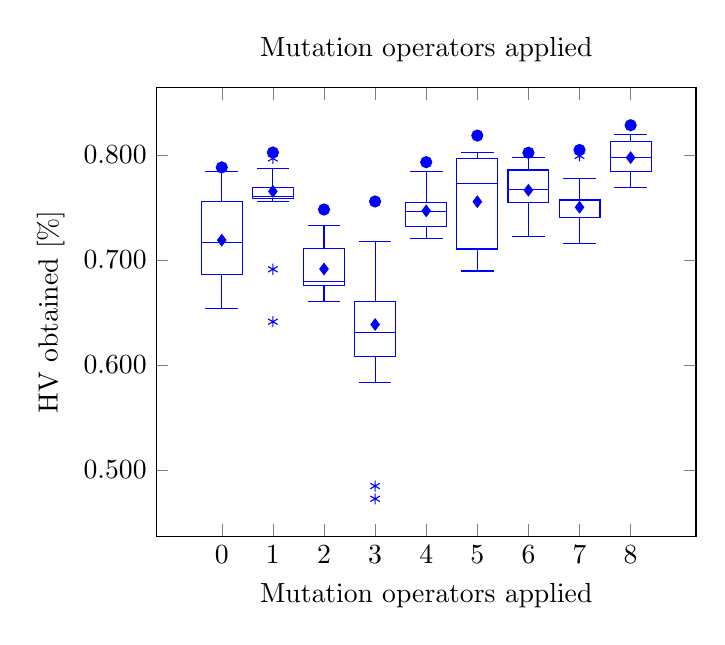
\begin{tikzpicture} 
\begin{axis}[ 
title={Mutation operators applied}, 
boxplot/draw direction=y, 
xtick={1,2,3,4,5,6,7,8,9}, 
xticklabels={0,1,2,3,4,5,6,7,8}, 
x tick label style={rotate=0, align=center}, 
xlabel={Mutation operators applied}, 
y tick label style={/pgf/number format/.cd,fixed,precision=3, zerofill}, 
ylabel={HV obtained [\%]}, 
] 

% ############## Mutations_AMALGAM_every_n=0 ################## 
\addplot[boxplot, mark=asterisk, 
boxplot prepared={ 
lower whisker=0.65389, 
upper whisker=0.78449, 
lower quartile=0.68608, 
upper quartile=0.7555, 
median=0.71645, 
average=0.71874}, 
color = blue, solid, area legend] 
coordinates {}; 
\addplot[only marks,mark=*,color = blue]coordinates{(1,0.78802)}; 

% ############## Mutations_AMALGAM_every_n=1 ################## 
\addplot[boxplot, mark=asterisk, 
boxplot prepared={ 
lower whisker=0.75567, 
upper whisker=0.78697, 
lower quartile=0.75806, 
upper quartile=0.7685, 
median=0.76063, 
average=0.7652}, 
color = blue, solid, area legend] 
coordinates {
(2,0.79658)
(2,0.69098)
(2,0.64105)}; 
\addplot[only marks,mark=*,color = blue]coordinates{(2,0.80221)}; 

% ############## Mutations_AMALGAM_every_n=2 ################## 
\addplot[boxplot, mark=asterisk, 
boxplot prepared={ 
lower whisker=0.66043, 
upper whisker=0.73228, 
lower quartile=0.6759, 
upper quartile=0.71108, 
median=0.67922, 
average=0.69122}, 
color = blue, solid, area legend] 
coordinates {}; 
\addplot[only marks,mark=*,color = blue]coordinates{(3,0.74786)}; 

% ############## Mutations_AMALGAM_every_n=3 ################## 
\addplot[boxplot, mark=asterisk, 
boxplot prepared={ 
lower whisker=0.58353, 
upper whisker=0.71751, 
lower quartile=0.6082, 
upper quartile=0.65997, 
median=0.63094, 
average=0.63836}, 
color = blue, solid, area legend] 
coordinates {
(4,0.47233)
(4,0.48451)}; 
\addplot[only marks,mark=*,color = blue]coordinates{(4,0.75555)}; 

% ############## Mutations_AMALGAM_every_n=4 ################## 
\addplot[boxplot, mark=asterisk, 
boxplot prepared={ 
lower whisker=0.72068, 
upper whisker=0.78376, 
lower quartile=0.73157, 
upper quartile=0.75468, 
median=0.74641, 
average=0.74662}, 
color = blue, solid, area legend] 
coordinates {}; 
\addplot[only marks,mark=*,color = blue]coordinates{(5,0.793)}; 

% ############## Mutations_AMALGAM_every_n=5 ################## 
\addplot[boxplot, mark=asterisk, 
boxplot prepared={ 
lower whisker=0.6893, 
upper whisker=0.80195, 
lower quartile=0.71031, 
upper quartile=0.7966, 
median=0.77244, 
average=0.75532}, 
color = blue, solid, area legend] 
coordinates {}; 
\addplot[only marks,mark=*,color = blue]coordinates{(6,0.81832)}; 

% ############## Mutations_AMALGAM_every_n=6 ################## 
\addplot[boxplot, mark=asterisk, 
boxplot prepared={ 
lower whisker=0.72242, 
upper whisker=0.79762, 
lower quartile=0.75485, 
upper quartile=0.78549, 
median=0.76658, 
average=0.76628}, 
color = blue, solid, area legend] 
coordinates {}; 
\addplot[only marks,mark=*,color = blue]coordinates{(7,0.80192)}; 

% ############## Mutations_AMALGAM_every_n=7 ################## 
\addplot[boxplot, mark=asterisk, 
boxplot prepared={ 
lower whisker=0.71571, 
upper whisker=0.77759, 
lower quartile=0.73995, 
upper quartile=0.75698, 
median=0.75626, 
average=0.75004}, 
color = blue, solid, area legend] 
coordinates {
(8,0.799)}; 
\addplot[only marks,mark=*,color = blue]coordinates{(8,0.80459)}; 

% ############## Mutations_AMALGAM_every_n=8 ################## 
\addplot[boxplot, mark=asterisk, 
boxplot prepared={ 
lower whisker=0.76866, 
upper whisker=0.81934, 
lower quartile=0.78378, 
upper quartile=0.81284, 
median=0.79763, 
average=0.79736}, 
color = blue, solid, area legend] 
coordinates {}; 
\addplot[only marks,mark=*,color = blue]coordinates{(9,0.82816)}; 

\end{axis}
\end{tikzpicture}
\end{figure} 

% ######################## UTRP SA Mutation operators applied ######################## 
\begin{figure} 
\centering 
\tikzsetnextfilename{UTRP_DBMOSA_BP_mutation_funcs_Counts_normal} 
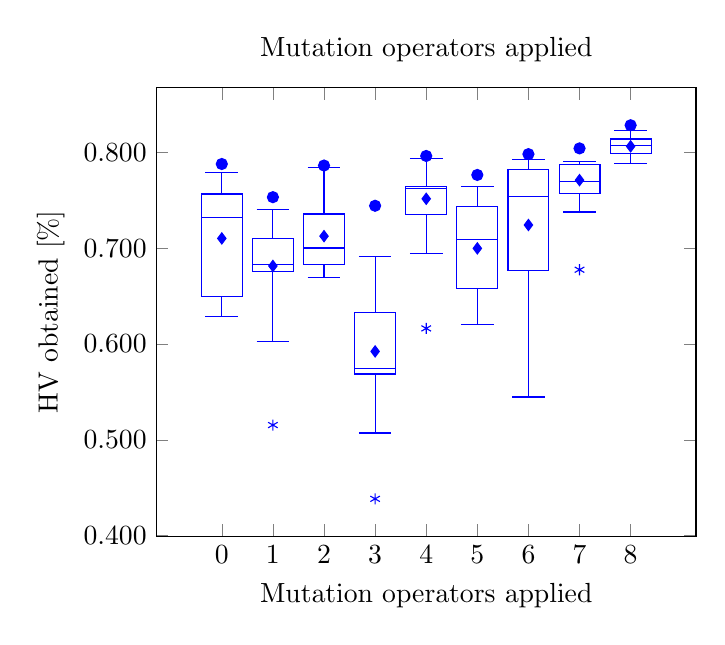
\begin{tikzpicture} 
\begin{axis}[ 
title={Mutation operators applied}, 
boxplot/draw direction=y, 
xtick={1,2,3,4,5,6,7,8,9}, 
xticklabels={0,1,2,3,4,5,6,7,8}, 
x tick label style={rotate=0, align=center}, 
xlabel={Mutation operators applied}, 
y tick label style={/pgf/number format/.cd,fixed,precision=3, zerofill}, 
ylabel={HV obtained [\%]}, 
] 

% ############## Mutations_Counts_normal=0 ################## 
\addplot[boxplot, mark=asterisk, 
boxplot prepared={ 
lower whisker=0.6289, 
upper whisker=0.77893, 
lower quartile=0.64949, 
upper quartile=0.75644, 
median=0.73149, 
average=0.71008}, 
color = blue, solid, area legend] 
coordinates {}; 
\addplot[only marks,mark=*,color = blue]coordinates{(1,0.78773)}; 

% ############## Mutations_Counts_normal=1 ################## 
\addplot[boxplot, mark=asterisk, 
boxplot prepared={ 
lower whisker=0.60252, 
upper whisker=0.73995, 
lower quartile=0.67515, 
upper quartile=0.71025, 
median=0.68305, 
average=0.68138}, 
color = blue, solid, area legend] 
coordinates {
(2,0.51539)}; 
\addplot[only marks,mark=*,color = blue]coordinates{(2,0.75313)}; 

% ############## Mutations_Counts_normal=2 ################## 
\addplot[boxplot, mark=asterisk, 
boxplot prepared={ 
lower whisker=0.66921, 
upper whisker=0.78377, 
lower quartile=0.6831, 
upper quartile=0.73551, 
median=0.70013, 
average=0.71247}, 
color = blue, solid, area legend] 
coordinates {}; 
\addplot[only marks,mark=*,color = blue]coordinates{(3,0.78613)}; 

% ############## Mutations_Counts_normal=3 ################## 
\addplot[boxplot, mark=asterisk, 
boxplot prepared={ 
lower whisker=0.50711, 
upper whisker=0.69107, 
lower quartile=0.5686, 
upper quartile=0.63234, 
median=0.57397, 
average=0.59218}, 
color = blue, solid, area legend] 
coordinates {
(4,0.4384)}; 
\addplot[only marks,mark=*,color = blue]coordinates{(4,0.74415)}; 

% ############## Mutations_Counts_normal=4 ################## 
\addplot[boxplot, mark=asterisk, 
boxplot prepared={ 
lower whisker=0.69392, 
upper whisker=0.79316, 
lower quartile=0.73491, 
upper quartile=0.76383, 
median=0.76194, 
average=0.75145}, 
color = blue, solid, area legend] 
coordinates {
(5,0.6162)}; 
\addplot[only marks,mark=*,color = blue]coordinates{(5,0.79611)}; 

% ############## Mutations_Counts_normal=5 ################## 
\addplot[boxplot, mark=asterisk, 
boxplot prepared={ 
lower whisker=0.62038, 
upper whisker=0.7645, 
lower quartile=0.65756, 
upper quartile=0.74382, 
median=0.70934, 
average=0.6997}, 
color = blue, solid, area legend] 
coordinates {}; 
\addplot[only marks,mark=*,color = blue]coordinates{(6,0.77631)}; 

% ############## Mutations_Counts_normal=6 ################## 
\addplot[boxplot, mark=asterisk, 
boxplot prepared={ 
lower whisker=0.54466, 
upper whisker=0.79277, 
lower quartile=0.67635, 
upper quartile=0.7817, 
median=0.7536, 
average=0.72407}, 
color = blue, solid, area legend] 
coordinates {}; 
\addplot[only marks,mark=*,color = blue]coordinates{(7,0.79802)}; 

% ############## Mutations_Counts_normal=7 ################## 
\addplot[boxplot, mark=asterisk, 
boxplot prepared={ 
lower whisker=0.73766, 
upper whisker=0.79054, 
lower quartile=0.75728, 
upper quartile=0.78691, 
median=0.76928, 
average=0.77094}, 
color = blue, solid, area legend] 
coordinates {
(8,0.67742)}; 
\addplot[only marks,mark=*,color = blue]coordinates{(8,0.80403)}; 

% ############## Mutations_Counts_normal=8 ################## 
\addplot[boxplot, mark=asterisk, 
boxplot prepared={ 
lower whisker=0.78859, 
upper whisker=0.82303, 
lower quartile=0.79904, 
upper quartile=0.8138, 
median=0.80677, 
average=0.80617}, 
color = blue, solid, area legend] 
coordinates {}; 
\addplot[only marks,mark=*,color = blue]coordinates{(9,0.82817)}; 

\end{axis}
\end{tikzpicture}
\end{figure} 
\begin{table}
\centering
\caption{Legend for the boxplot.}
\begin{tabular}{ll}
\toprule
 Index &                                               Name \\
\midrule
     0 &               [MSC\_add\_terminal, MSC\_del\_terminal] \\
     1 &                        [Add\_vertex, Delete\_vertex] \\
     2 &       [Trim\_one\_terminal\_cb, Grow\_one\_terminal\_cb] \\
     3 &       [Insert\_inside\_vertex, Delete\_inside\_vertex] \\
     4 & [Add\_vertex, Delete\_vertex, Insert\_inside\_verte... \\
     5 &        [Add\_vertex, Delete\_vertex, Intertwine\_two] \\
     6 & [Add\_vertex, Delete\_vertex, Insert\_inside\_verte... \\
     7 & [MSC\_add\_terminal, MSC\_del\_terminal, Insert\_ins... \\
     8 & [Add\_vertex, Delete\_vertex, Insert\_inside\_verte... \\
\bottomrule
\end{tabular}
\end{table}

\end{document}
